% Self-contained LaTeX reconstruction from the original editable report.
% Compile: pdflatex -interaction=nonstopmode -halt-on-error Quantum_Precision_Heat_Tradeoff_Report.tex
% Compatible with pdfLaTeX under TeX Live 2025.
\documentclass[11pt,letterpaper]{article}
\usepackage[letterpaper,left=0.9in,right=0.9in,top=0.86in,bottom=0.86in,headheight=16pt,headsep=19pt,footskip=25pt]{geometry}
\usepackage[T1]{fontenc}
\usepackage[utf8]{inputenc}
\usepackage{libertinus}
\usepackage{orcidlink}
\usepackage{microtype}
\usepackage{amsmath,mathtools}
\usepackage{booktabs,tabularx,array}
\usepackage{needspace}
\usepackage{titlesec}
\usepackage{xcolor}
\usepackage{tikz}
\usepackage{pgfplots}
\pgfplotsset{compat=1.18}
\usepackage{fancyhdr}
\usepackage{hyperref}
\definecolor{teal}{HTML}{175269}
\definecolor{ink}{HTML}{172734}
\definecolor{graytext}{HTML}{5B6770}
\hypersetup{pdftitle={Quantum Precision--Heat Tradeoff Report},pdfsubject={A self-contained explanation of the physical model, proof, and result},pdfauthor={Ranyiliu Chen; Ruge Lin},colorlinks=true,linkcolor=teal,urlcolor=teal}
\setlength{\parindent}{0pt}
\setlength{\parskip}{3.7pt plus 1.1pt minus 0.8pt}
\linespread{1.03}
\raggedbottom
\setlength{\emergencystretch}{2em}
\setcounter{secnumdepth}{2}
\setcounter{tocdepth}{2}
\titleformat{\section}[block]{\color{teal}\sffamily\bfseries\fontsize{16}{19}\selectfont}{\thesection}{0.85em}{}
\titlespacing*{\section}{0pt}{16pt plus 3pt minus 1pt}{5pt plus 1pt}
\titleformat{\subsection}[block]{\sffamily\bfseries\fontsize{12.5}{15}\selectfont\color{ink}}{\thesubsection}{0.65em}{}
\titleformat{\subsubsection}[block]{\sffamily\bfseries\small\color{ink}}{}{0pt}{}
\titlespacing*{\subsubsection}{0pt}{9pt plus 1pt minus 1pt}{2pt}
\titlespacing*{\subsection}{0pt}{11pt plus 2pt minus 1pt}{3pt}
\fancyhf{}
\fancyhead[L]{\footnotesize\sffamily\color{graytext}QUANTUM PRECISION--HEAT TRADEOFF}
\fancyhead[R]{\footnotesize\sffamily\color{graytext}EXPLANATORY REPORT}
\fancyfoot[C]{\footnotesize\sffamily\color{graytext}\thepage}
\renewcommand{\headrulewidth}{0.35pt}
\renewcommand{\footrulewidth}{0pt}
\pagestyle{fancy}
\allowdisplaybreaks[1]
\AtBeginDocument{\color{ink}}
\begin{document}
{\sffamily\bfseries\color{ink}\fontsize{22}{27}\selectfont Quantum Precision--Heat Tradeoff Report\par}
\vspace{3pt}
{\sffamily\small\color{graytext}A self-contained explanation of the physical model, proof, and result\par}
\vspace{7pt}
{\sffamily\small\color{ink}Ranyiliu Chen\,\orcidlink{0000-0001-6060-6192}\qquad Ruge Lin\,\orcidlink{0000-0002-9297-7622}\par}
{\sffamily\footnotesize\color{graytext}
Quantum Science Center of Guangdong-Hong Kong-Macao Greater Bay Area, Shenzhen 518045, China\par
Thrust of Artificial Intelligence, Information Hub, The Hong Kong University of Science and Technology (Guangzhou), Guangzhou 511453, China\par
Corresponding author: \href{mailto:ranyiliu.chen@outlook.com}{ranyiliu.chen@outlook.com}\par}
\vspace{7pt}
\noindent\color{teal}\rule{\linewidth}{0.85pt}\color{ink}
\vspace{4pt}



A device can change its average output only slightly and still have a heat cost that remains large. The reason is that it must produce the correct output for each possible input. That requirement can force information into its surroundings even when the average output hardly changes.

We study a precise version of this problem. A device receives one of two perfectly distinguishable quantum states. It must produce the corresponding member of a pair that are slightly less distinguishable. We determine the least mean heat that can be approached when both the change and the permitted error become small. The answer depends on the error divided by the square of the target overlap.

The argument begins with a working device. It then establishes a lower bound for every allowed device, improves the construction until the two bounds meet, and explains the consequences. The five parts below contain sixteen connected steps, from the first working device to the complete theorem. Each step introduces the background needed to understand what comes next.

\vspace{3pt}
\begingroup
\setlength{\parskip}{0pt}
\small
\tableofcontents
\endgroup
\clearpage

\Needspace{10\baselineskip}
\section{A working device and the precision scale}\label{sec:device}

\Needspace{7\baselineskip}
\subsection{A finite device that passes both output tests}\label{subsec:finite-device}

\Needspace{5\baselineskip}
\subsubsection{States and accuracy}\label{states-and-accuracy}

A \textbf{qubit} is a quantum system with two basic alternatives, written \(\left| 0 \right\rangle\) and \(\left| 1 \right\rangle\). The brackets identify a state vector. These two states can be distinguished perfectly by a suitable measurement. We call them orthogonal.

A pure state can also be a combination \(a_{0}\left| 0 \right\rangle + a_{1}\left| 1 \right\rangle\). The numbers \(a_{0},a_{1}\) are amplitudes. Their squared magnitudes, \(\left| a_{0} \right|^{2}\) and \(\left| a_{1} \right|^{2}\), give the probabilities of the two answers in a zero-or-one measurement, and add to one. Amplitudes can be complex numbers. A complex number has a real part and an imaginary part; its magnitude is the square root of the sum of their squares. A square root is the nonnegative number whose square equals its argument. Signs and complex phases affect other measurements, so amplitudes contain more information than these two probabilities.

A vector's length is the square root of the sum of its squared amplitude magnitudes. State vectors have length one and are therefore called unit vectors.

To compare two vectors, multiply their matching amplitudes, taking the complex conjugate of each amplitude from the first vector, and add. Complex conjugation reverses the sign of the imaginary part. The result is their \textbf{inner product}. Zero inner product means orthogonality; its magnitude is their overlap. A measurement can use any complete set of orthogonal unit vectors as its alternatives. For a pure input, the probability of each answer is the squared magnitude of its inner product with that alternative. A linear operation acts on a combination by acting on each term separately.

A \textbf{pure state} has one state vector as its complete description. A \textbf{mixed state} is a probabilistic mixture of pure states. Both can be represented by a density matrix: a table that determines the probabilities of every possible measurement. For a qubit, write

\[\rho = \begin{pmatrix}
p & z \\
z^{*} & 1 - p
\end{pmatrix}.\]

The letter \(\rho\) names the state. The diagonal entries give the zero-or-one probabilities. The off-diagonal number \(z\) is called coherence; it describes interference between the alternatives. The star means complex conjugation, which reverses the sign of the imaginary part. An eigenvector is a direction that a matrix only multiplies by a number; that number is its eigenvalue. For a density matrix, the eigenvalues are nonnegative and sum to one. They are the probabilities in a mixture of mutually orthogonal pure states.

For a pure vector, its density matrix is obtained by multiplying each amplitude by each conjugated amplitude:

\[a_{0}\left| 0 \right\rangle + a_{1}\left| 1 \right\rangle\quad \leftrightarrow \quad\begin{pmatrix}
\left| a_{0} \right|^{2} & a_{0}a_{1}^{*} \\
a_{1}a_{0}^{*} & \left| a_{1} \right|^{2}
\end{pmatrix}.\]

To form a probabilistic mixture, multiply each component's density matrix by its probability and add. This rule will let us calculate the device's outputs directly.

A concrete example shows why a combination of amplitudes differs from a probabilistic mixture. Define

\[\left| + \right\rangle = \frac{\left| 0 \right\rangle + \left| 1 \right\rangle}{\sqrt{2}},\quad\quad\left| - \right\rangle = \frac{\left| 0 \right\rangle - \left| 1 \right\rangle}{\sqrt{2}}.\]

\Needspace{8\baselineskip}
Both give zero and one with equal probabilities in the original measurement. Yet their inner product is \((1 - 1)/2 = 0\), so a measurement with alternatives plus and minus distinguishes them perfectly. The state \(\left| + \right\rangle\) always gives plus. A fifty-fifty mixture of \(\left| 0 \right\rangle\) and \(\left| 1 \right\rangle\) gives plus only half the time, because each component has squared overlap \(1/2\) with \(\left| + \right\rangle\). The off-diagonal entries distinguish these situations even when their zero-or-one probabilities agree.

A useful picture represents a qubit state by a point inside a sphere of radius one. This point is its \textbf{Bloch vector}. In terms of the matrix above, its three coordinates are

\[(2\operatorname{Re}z,\, - 2\operatorname{Im}z,\, 2p - 1).\]

Here \(Re\) and \(Im\) mean real and imaginary part. Pure states lie on the sphere's surface. Mixed states lie inside it. The inputs \(\left| 0 \right\rangle\) and \(\left| 1 \right\rangle\) are the north and south poles. The center represents equal uncertainty between them. Coordinates provide a picture of a state, not the physical location of a particle.

Let \(x\) be the input label: either zero or one, each with probability one half. The desired output on branch \(x\) is \(\phi_{x}\). A branch means all runs with that same input. Choose \(0 < s < 1\) and define \(c = \sqrt{1 - s^{2}}\). Our targets have Bloch vectors

\[\phi_{0}:\ ( - s,0,c),\quad\quad\phi_{1}:\ ( - s,0, - c).\]

Both are pure because \(s^{2} + c^{2} = 1\). Each moves sideways by the same amount. For small \(s\), one remains near the north pole and the other near the south pole. The magnitude of their state-vector overlap is \(s\). Overlap zero means perfect distinguishability. An overlap strictly between zero and one means distinct states that cannot always be distinguished without error.

For later calculations the target matrices are

\[\phi_{0} = \begin{pmatrix}
(1 + c)/2 & - s/2 \\
 - s/2 & (1 - c)/2
\end{pmatrix},\quad\quad\phi_{1} = \begin{pmatrix}
(1 - c)/2 & - s/2 \\
 - s/2 & (1 + c)/2
\end{pmatrix}.\]

Call the actual output \(\sigma_{x}\). We compare states using \textbf{trace distance}, written \(D(\rho,\sigma)\). Operationally, it is the largest difference between the probabilities that the two states assign to the same measurement event. For qubits, it is half the ordinary distance between their Bloch vectors. Its general formula is

\[D(\rho,\sigma) = \frac{1}{2} \lVert \rho - \sigma\rVert_{1}.\]

The difference of two density matrices is Hermitian: exchanging rows and columns and taking complex conjugates leaves it unchanged. For such a matrix, the trace norm \(\lVert \cdot\rVert_{1}\) is the sum of the absolute values of its eigenvalues. These are the matrices on which we use the trace norm in this report. Our tolerance \(\epsilon\) must satisfy

\[0 < \epsilon < c/2,\quad\quad D\left( \sigma_{0},\phi_{0} \right) \leq \epsilon,\quad\quad D\left( \sigma_{1},\phi_{1} \right) \leq \epsilon.\]

The sign \(\leq\) means no greater than. Each output must pass its own test. The cutoff \(c/2\) keeps the requirement stronger than merely preparing the average target. That average has Bloch vector \(( - s,0,0)\), halfway between the two targets, and trace distance \(c/2\) from each. Our smaller error therefore rules out a device that always produces this same average state.

\Needspace{5\baselineskip}
\subsubsection{The complete apparatus and its heat}\label{the-complete-apparatus-and-its-heat}

The input and output qubit is called \(S\). A finite internal workspace is called \(A\). The complete thermal reservoir, also called the bath, is \(B\). Finite means that each has a finite number of independent quantum directions. The initial workspace state \(\tau_{A}\) can be arbitrary. The initial bath state \(\gamma_{B}\) must be a Gibbs state: thermal equilibrium at a positive temperature \(T\) with finite energy levels.

Input, workspace, and bath initially have no correlations. One fixed \textbf{unitary} acts on them together. A unitary is a linear reversible quantum transformation; it preserves lengths and inner products of state vectors. The same operation must handle either input. Its controls receive no separate copy of the unknown label. Predetermined driving can supply or recover work, so the operation need not preserve the energy of the uncoupled components.

Energy assignments, called Hamiltonians, are unchanged between the beginning and end, and interactions are switched off at those boundaries. The system's boundary Hamiltonian is zero. These conditions make the energy account precise; the relation between heat and supplied work is explained in Section~\ref{subsec:contribution}.

The workspace must return to its initial state after averaging the two branches. If \(\rho\prime_{A,x}\) denotes its final state on branch \(x\), the return condition is

\[\frac{\rho\prime_{A,0} + \rho\prime_{A,1}}{2} = \tau_{A}.\]

A prime means final. A \textbf{marginal} is the state of one part when we ignore the other parts. Only this average workspace marginal must return. The two branch marginals may differ, and final correlations may remain. Thus this condition alone does not guarantee independent reuse on arbitrary future inputs.

Heat \(Q\) is the mean energy gained by the entire bath. Every fresh and spent thermal component counts. We measure it in the dimensionless units

\[q = \frac{Q}{k_{\mathrm{B}}T\ln 2}.\]

The constant \(k_{\mathrm{B}}\) converts temperature to energy, and \(\ln 2 \approx 0.693147\) is the natural logarithm of two. One unit of \(q\) is therefore the energy \(k_{\mathrm{B}}T\ln 2\). Positive heat means the bath gains energy. The input source and the construction of the controller lie outside this accounting. The result concerns one processed input, even if the device uses many successive interactions.

\Needspace{5\baselineskip}
\subsubsection{A complete working example}\label{a-complete-working-example}

We first use no workspace and only one bath qubit. Its two energy levels are zero and \(\Delta\). We design the output backward from the target matrix: keep the off-diagonal entry exactly correct and use the permitted error only in the diagonal probabilities.

The target's opposite-basis probability is \((1 - c)/2\). We choose the actual probability \(u\) to be this value plus \(\epsilon\). The amplitudes \(C\) and \(v\) will produce probabilities \(1 - u\) and \(u\). Let \(b\) be the probability of bath state zero minus the probability of bath state one. Our operation will make these bath alternatives contribute coherences \(- Cv\) and \(+ Cv\). Their average is \(- bCv\), which must equal the target entry \(- s/2\). These choices give

\[u = \frac{1 - c}{2} + \epsilon,\quad\quad C = \sqrt{1 - u},\quad\quad v = \sqrt{u},\quad\quad b = \frac{s}{2Cv}.\]

Here \(C\) and \(v\) are amplitudes, and \(b\) is the bath's population bias. Choose the bath probabilities

\[p_{0} = \frac{1 + b}{2},\quad\quad p_{1} = \frac{1 - b}{2},\quad\quad\frac{\Delta}{k_{\mathrm{B}}T\ln 2} = \log_{2}\frac{1 + b}{1 - b}.\]

\clearpage
The expression \(\log_{2}y\) is the power to which two must be raised to give \(y\). This gap is exactly the Gibbs condition: the upper level is less likely by the thermal factor determined by its energy. Because \((1 - c)/2 < u < 1/2\), we have \(0 < b < 1\). Both probabilities are positive and the energy gap is finite. To check the upper bound on \(b\), note that \(u(1 - u)\) increases below \(1/2\) and equals \(s^{2}/4\) at \(u = (1 - c)/2\).

The following four rules specify the operation. In \(\left| x,y \right\rangle\), the first entry is the system and the second is the bath. Adjacent state vectors on the right describe their combined state.

\[\begin{matrix}
\left| 0,0 \right\rangle & \mapsto \left( C\left| 0 \right\rangle - v\left| 1 \right\rangle \right)\left| 0 \right\rangle, \\
\left| 0,1 \right\rangle & \mapsto \left( C\left| 0 \right\rangle + v\left| 1 \right\rangle \right)\left| 1 \right\rangle, \\
\left| 1,0 \right\rangle & \mapsto \left( - v\left| 0 \right\rangle + C\left| 1 \right\rangle \right)\left| 1 \right\rangle, \\
\left| 1,1 \right\rangle & \mapsto \left( v\left| 0 \right\rangle + C\left| 1 \right\rangle \right)\left| 0 \right\rangle.
\end{matrix}\]

Each output has length one, and the four outputs are mutually orthogonal. Where two bath states agree, the corresponding system inner product is \(Cv - vC = 0\); where the bath states differ, they already supply orthogonality. Thus the rules define an allowed unitary. They can be implemented by a joint rotation followed by a controlled bath flip. No input label is handed to an external controller.

Average over the two initial bath possibilities with weights \(p_{0},p_{1}\). The system outputs are

\[\sigma_{0} = \begin{pmatrix}
1 - u & - s/2 \\
 - s/2 & u
\end{pmatrix},\quad\quad\sigma_{1} = \begin{pmatrix}
u & - s/2 \\
 - s/2 & 1 - u
\end{pmatrix}.\]

The off-diagonal entry is correct because \(\left( p_{1} - p_{0} \right)Cv = - bCv = - s/2\). The diagonal entries differ from their targets by exactly \(\epsilon\). The difference matrix has eigenvalues \(+ \epsilon\) and \(- \epsilon\), so each trace distance is exactly \(\epsilon\).

On input zero the bath probabilities stay unchanged. On input one they interchange. Their average is therefore \((1/2,1/2)\). The mean upper-level probability has increased by \(b/2\), giving

\[Q_{\mathrm{bare}} = \frac{b\Delta}{2},\quad\quad q_{\mathrm{bare}} = \frac{b}{2}\log_{2}\frac{1 + b}{1 - b}.\]

The subscript ``bare'' means this first collision without later recovery. We now have a complete finite device, its two errors, and its heat. This is an achievable cost. Establishing the least possible cost requires an argument about every allowed apparatus.

\Needspace{7\baselineskip}
\subsection{Why squared overlap sets the precision scale}\label{subsec:squared-overlap}

\textbf{Preliminary.} A limit describes what happens along a sequence. The notation \(s \rightarrow 0\) means that positive values of \(s\) become arbitrarily small. The approximation symbol \(\approx\) below concerns this small-\(s\) regime.

The target's sideways displacement is \(s\), but its probability of the opposite zero-or-one answer is

\[\frac{1 - c}{2} = \frac{s^{2}}{2(1 + c)} \approx \frac{s^{2}}{4}.\]

The equality follows by multiplying \(1 - c\) by \((1 + c)/(1 + c)\) and using \(1 - c^{2} = s^{2}\). The approximation follows because \(c \rightarrow 1\). The displacement along the surface therefore has two scales: a sideways coherence of size \(s\) and a probability change of size \(s^{2}\).

\Needspace{6\baselineskip}
The device preserves the sideways component exactly. Its allowed extra mixing enters through \(u = (1 - c)/2 + \epsilon\). Thus the competition is between \(s^{2}/4\) and \(\epsilon\). If their ratio approaches a finite nonnegative number \(r\), then

\[\frac{\epsilon}{s^{2}} \rightarrow r,\quad\quad\frac{u}{s^{2}} \rightarrow \frac{1}{4} + r,\quad\quad b = \frac{s}{2\sqrt{u(1 - u)}} \rightarrow \frac{1}{\sqrt{1 + 4r}}.\]

For example, both \(\epsilon = s^{2}\) and \(\epsilon = s^{3}\) are much smaller than \(s\) at small \(s\). Yet their ratios to \(s^{2}\) approach one and zero. They impose different demands on the thermal bias.

This geometry explains why squared overlap is the candidate precision scale. It does not yet show that all other devices must respect the same heat law. The following analysis supplies that universal argument.

\Needspace{10\baselineskip}
\section{From output accuracy to environmental information}\label{sec:information}

\Needspace{7\baselineskip}
\subsection{What accuracy requires from every device}\label{subsec:output-accuracy}

\textbf{Preliminary.} A bound is a limit on what a quantity can be. Here we extract two bounds directly from the output tests, without assuming any particular circuit or bath.

Let \(\delta_{0}\) be the probability of obtaining answer one from output \(\sigma_{0}\), and let \(\delta_{1}\) be the probability of obtaining answer zero from output \(\sigma_{1}\). These are wrong-basis probabilities, not the complete output errors. Let \(a_{x}\) be the upper off-diagonal entry of \(\sigma_{x}\).

Each target has wrong-basis probability \((1 - c)/2\) and off-diagonal entry \(- s/2\). Trace distance limits each probability error by \(\epsilon\). It also limits the off-diagonal error: a traceless Hermitian difference with entries \(h,z,z^{*}, - h\) has eigenvalues \(\pm \sqrt{h^{2} + |z|^{2}}\), so its trace distance is at least \(|z|\). Consequently,

\[\delta_{x} \leq d,\quad\quad\left| a_{x} + s/2 \right| \leq \epsilon,\quad\quad d = \frac{1 - c}{2} + \epsilon.\]

The symbol \(d\) is a convenient common upper bound; it need not equal either actual probability. It equals the construction's parameter \(u\). Define their mean as \(\overline{\delta} = \left( \delta_{0} + \delta_{1} \right)/2\). Adding the two off-diagonal errors gives

\[\overline{\delta} \leq d,\quad\quad\left| a_{0} + a_{1} \right| \geq s - 2\epsilon.\]

Thus every accurate device must create a common coherence of almost size \(s\) while allowing only a small probability of the opposite basis answer. Both branch tests are needed to draw this conclusion.

\Needspace{7\baselineskip}
\subsection{Describing every allowed reversible interaction}\label{subsec:arbitrary-unitary}

\textbf{Preliminary.} Matrices represent linear transformations. Multiplication means applying them in sequence, with the rightmost operation first. The identity \(I\) changes nothing. A dagger, as in \(K^{\dagger}\), means conjugate transpose. A Hermitian matrix is positive when its eigenvalues are nonnegative. A matrix inequality means that the right-hand matrix minus the left-hand matrix is positive; it is not an entry-by-entry comparison. A positive matrix's square root replaces each eigenvalue by its nonnegative square root. The trace \(Tr\) is the sum of diagonal entries.

Combine workspace and bath into the complete environment \(E = AB\). Their initial independent state is \(\Omega = \tau_{A} \otimes \gamma_{B}\). The tensor-product sign \(\otimes\) combines descriptions of separate systems. For initially independent parts, it combines their probabilities by multiplication.

\clearpage
We can write any unitary on a qubit and a finite environment in the form

\[U = \begin{pmatrix}
V_{0}C_{0} & - V_{0}K^{\dagger} \\
V_{1}K & V_{1}C_{1}
\end{pmatrix},\quad\quad C_{0} = \sqrt{I - K^{\dagger}K},\quad C_{1} = \sqrt{I - KK^{\dagger}}.\]

The two columns correspond to input zero or one; the two rows correspond to output zero or one. Each entry is itself an environment matrix. This two-by-two array does not limit the environment to two states. The diagonal blocks describe remaining in the same system basis state. The other blocks describe changing it. The matrices \(V_{0},V_{1}\) are environment unitaries, and \(K\) is a contraction: it cannot increase a vector's length.

The mathematical fact behind this form is the complete cosine--sine decomposition. It breaks a unitary into independent two-direction rotations and changes of basis. In each rotation, the squared survival and transition amplitudes add to one. Grouping those amplitudes gives \(C_{0},C_{1},K\). Rotations with zero or complete transition are included. No block has to be inverted, so singular blocks and initial states with zero eigenvalues remain covered. This is a description of every allowed unitary, not a restriction to the first working-device example.

Define two comparison environment states and a transformed transition matrix:

\[\tau_{0} = V_{0}\Omega V_{0}^{\dagger},\quad\quad\tau_{1} = V_{1}\Omega V_{1}^{\dagger},\quad\quad G = V_{1}KV_{0}^{\dagger}.\]

These comparison states describe the environment transformations with the survival factors replaced by \(I\). They are mathematical comparison objects; they are not generally the actual outputs. Define the complex number

\[\ell = \operatorname{Tr}\left\lbrack \left( \tau_{0} - \tau_{1} \right)G^{\dagger} \right\rbrack.\]

It measures how their difference couples to the transition. A basis-change probability comes from the squared size of the changing-state block. Coherence comes from combining a staying-state amplitude with a changing-state amplitude. Applying these rules to the displayed blocks gives

\[\delta_{0} = \operatorname{Tr}\left( \tau_{0}G^{\dagger}G \right),\quad\quad\delta_{1} = \operatorname{Tr}\left( \tau_{1}GG^{\dagger} \right),\quad\quad\left| \ell - a_{0} - a_{1} \right| \leq \delta_{0} + \delta_{1}.\]

Why is the last error so small? Replacing \(C_{0}\) by \(I\) produces a term containing both a transition factor and \(I - C_{0}\). The matrix inequality \(\left( I - C_{0} \right)^{2} \leq K^{\dagger}K\) says that the squared survival change is no greater than the transition probability operator. Cauchy--Schwarz, the rule bounding an inner product by the product of lengths, then bounds this replacement error by \(\delta_{0}\). The other branch contributes at most \(\delta_{1}\).

Combining this with the two output-accuracy bounds gives

\[|\ell| \geq [s-2\epsilon-2d]_{+},\quad\quad[y]_{+} = \max\{ y,0\}.\]

The maximum selects the larger argument. This notation replaces a negative proposed lower bound by zero. If the comparison states were identical, their difference would give \(\ell = 0\). The displayed bound rules this out whenever \(s > 2\epsilon + 2d\). Along the limit studied here, \(\epsilon/s\) and \(d/s\) both approach zero, so that condition eventually holds. Accurate outputs therefore force the comparison states to differ.

The correction is proportional to \(d\), which is of size \(s^{2}\) at a fixed ratio \(\epsilon/s^{2}\). A correction of size \(\sqrt{d}\) would be comparable to the coherence \(s\) and would lose the sharp information needed for the final result.

\Needspace{7\baselineskip}
\subsection{Why the environmental comparison states must differ}\label{subsec:spectral-separation}

\textbf{Preliminary.} A state can be described by its eigenvectors and eigenvalues: orthogonal directions and the probabilities assigned to them. Two density matrices may use different directions. A comparison must therefore include both their probabilities and the relation between their eigenvectors.

Both comparison states have the same list of eigenvalues as \(\Omega\), because their transformations are reversible. They can still place those probabilities in different directions. For example, assigning probabilities \(3/4,1/4\) to zero and one gives a different state from assigning \(1/4,3/4\). Equal eigenvalue lists do not make the states identical.

Let \(\lambda_{i}\) and \(\left| u_{i} \right\rangle\) be the eigenvalues and unit eigenvectors of \(\tau_{0}\). Let \(\mu_{j}\) and \(\left| v_{j} \right\rangle\) be those of \(\tau_{1}\). Indices \(i,j\) run over complete sets, including directions of zero probability. The inner product \(\langle u_{i} \mid v_{j}\rangle\) is the overlap of two vectors. Define its squared magnitude as \(w_{ij} = \left| \langle u_{i} \mid v_{j}\rangle \right|^{2}\).

Our measure of separation is

\[\mathcal{T} = \frac{1}{2}\sum_{i,j}^{}\frac{\left( \lambda_{i} - \mu_{j} \right)^{2}}{\lambda_{i} + \mu_{j}}\, w_{ij}.\]

The summation sign means add the term for every pair \(i,j\). If both probabilities are zero, that term is defined as zero. Each other term compares a squared probability difference with its total probability, weighted by the overlap of the directions. Every term is nonnegative. Also \(\left( \lambda_{i} - \mu_{j} \right)^{2} \leq \left( \lambda_{i} + \mu_{j} \right)^{2}\), and each row and column of \(w\) sums to one. Summing this upper bound gives \(\mathcal{T} \leq 1\). This number between zero and one is called spectral triangular discrimination. Its exact definition matters; a different measure of distinguishability cannot be substituted without a new argument.

To connect this separation to the outputs, put \(t_{ij} = \langle u_{i} \mid G^{\dagger} \mid v_{j}\rangle\). This means apply \(G^{\dagger}\) to \(\left| v_{j} \right\rangle\), then take the inner product with \(\left| u_{i} \right\rangle\). Expanding the trace in complete eigenvector sets gives

\[\ell = \sum_{i,j}^{}\left( \lambda_{i} - \mu_{j} \right)\langle v_{j} \mid u_{i}\rangle\, t_{ij}.\]

Apply the weighted Cauchy--Schwarz inequality. This is the same rule that bounds the square of a sum of products by the product of two sums of squares. Here its two factors are

\[2\mathcal{T}\quad\text{and}\quad\sum_{i,j}^{}\left( \lambda_{i} + \mu_{j} \right)\left| t_{ij} \right|^{2} = 2\overline{\delta}.\]

The second equality is exactly the sum of the two transition-probability formulas in the general-unitary calculation. Hence

\[|\ell|^{2} \leq 4\overline{\delta}\mathcal{T} \leq 4d\mathcal{T}.\]

Rare transitions make the factor \(d\) small. The output tests nevertheless require \(|\ell|\) to remain close to \(s\). Therefore the comparison states must have enough separation to compensate. Define

\[b_{\mathrm{low}} = \frac{[s-2\epsilon-2d]_{+}}{2\sqrt{d}}.\]

The subscript identifies this as a lower-bound parameter, distinct from the constructed bath bias \(b\).

\Needspace{6\baselineskip}
The conclusion is

\[\mathcal{T} \geq b_{\mathrm{low}}^{2}.\]

We have converted a requirement on the visible outputs into a necessary difference between two environment states used in the proof.

\Needspace{7\baselineskip}
\subsection{Why separation forces information about the input}\label{subsec:spectral-information}

\textbf{Preliminary.} Entropy measures uncertainty in bits. If a state \(\rho\) has eigenvalues \(\lambda_{i}\), define

\[H(\rho) = - \sum_{i}^{}\lambda_{i}\log_{2}\lambda_{i}.\]

The convention \(0\log_{2}0 = 0\) defines a zero-probability term. A pure state has entropy zero. This entropy describes the mixture represented by the state, rather than the randomness of every possible measurement. For example, \(\left| + \right\rangle\) is pure even though its zero-or-one measurement is random. An equal mixture of two orthogonal alternatives has entropy one bit. For a binary probability \(p\), it is useful to write

\[h_{2}(p) = - p\log_{2}p - (1 - p)\log_{2}(1 - p).\]

The subscript two specifies base-two logarithms. The uncertainty of a fair coin is \(h_{2}(1/2) = 1\); a certain answer has \(h_{2}(0) = h_{2}(1) = 0\).

For two equally likely quantum states \(\rho_{0},\rho_{1}\), define their \textbf{Holevo information} as

\[\chi\left( \rho_{0},\rho_{1} \right) = H\left( \frac{\rho_{0} + \rho_{1}}{2} \right) - \frac{H\left( \rho_{0} \right) + H\left( \rho_{1} \right)}{2}.\]

This is the extra uncertainty introduced by not knowing which state was prepared. It measures quantum information about the binary input label and lies between zero and one bit. It is zero for identical states and one for perfectly distinguishable states. In general, it is not a promise that one measurement will recover that many classical bits.

Consider two ordinary records of the input. The first always equals the input: its average is a fair zero-or-one value, but specifying the input makes the record certain. Its information is \(1 - 0 = 1\) bit. The second is an unrelated fair coin: it stays uncertain even after specifying the input, so its information is \(1 - 1 = 0\). Both records look equally random when averaged. The subtraction in \(\chi\) reveals which one carries information about the input.

We need the increasing function

\[J_{2}(b) = 1 - h_{2}\left( \frac{1 + b}{2} \right),\quad\quad 0 \leq b \leq 1.\]

It is the entropy deficit of a binary distribution with bias \(b\). At bias zero it equals zero; at bias one it equals one. The information step establishes

\[\chi\left( \tau_{0},\tau_{1} \right) \geq J_{2}\left( \sqrt{\mathcal{T}} \right) \geq J_{2}\left( b_{\mathrm{low}} \right).\]

\Needspace{5\baselineskip}
\subsubsection{Why the bound also covers different quantum bases}\label{why-the-bound-also-covers-different-quantum-bases}

Use the spectral weights from the spectral comparison above to make two ordinary probability arrays,

\[P_{ij} = \lambda_{i}w_{ij},\quad\quad Q_{ij} = \mu_{j}w_{ij}.\]

These arrays describe two calculations on paper. To generate \(P\), select \(i\) with probability \(\lambda_{i}\), then \(j\) with probability \(w_{ij}\). To generate \(Q\), select \(j\) with probability \(\mu_{j}\), then \(i\) with probability \(w_{ij}\). The row and column sums of \(w\) make both rules normalized. They compare the spectral descriptions without requiring the physical device to perform either procedure.

For ordinary distributions define \(\operatorname{JS}(P,Q)\) by the same entropy-difference formula used for \(\chi\). Here entropy is evaluated directly from the entries of each array. A general matrix entropy comparison gives

\[\chi\left( \tau_{0},\tau_{1} \right) \geq \operatorname{JS}(P,Q).\]

Its precise content can be seen by setting \(M = \left( \tau_{0} + \tau_{1} \right)/2\) and \(m_{ij} = \left( \lambda_{i} + \mu_{j} \right)/2\). The needed matrix fact is

\[H(M) \geq - \sum_{i,j}^{}w_{ij}m_{ij}\log_{2}m_{ij}.\]

Subtracting the mean entropy of the two original states from both sides gives the displayed information comparison. In the probability-array formula, the terms involving \(\log_{2}w_{ij}\) cancel. Zero-weight terms are understood by continuity.

The displayed matrix-entropy inequality is a background mathematical fact used here. If the states share an eigenbasis, choose the same eigenvectors for both. Then \(w_{ij}\) is one for matching directions and zero otherwise, and the inequality becomes an equality, entry by entry. The general theorem guarantees the stated direction even for noncommuting matrices, whose multiplication depends on order. Their quantum information is at least the information in these particular algebraic arrays. The following argument uses ordinary probabilities to obtain the binary heat curve.

\Needspace{5\baselineskip}
\subsubsection{Why this particular information curve appears}\label{why-this-particular-information-curve-appears}

On each cell with \(P_{ij} + Q_{ij} > 0\), define its average weight and signed bias as

\[\nu_{ij} = \frac{P_{ij} + Q_{ij}}{2},\quad\quad a_{ij} = \frac{P_{ij} - Q_{ij}}{P_{ij} + Q_{ij}}.\]

The weights add to one, and each bias lies between minus one and one. Zero-weight cells contribute nothing. Direct substitution into the definitions gives

\[\operatorname{JS}(P,Q) = \sum_{i,j}^{}\nu_{ij}J_{2}\left( a_{ij} \right),\quad\quad\mathcal{T} = \sum_{i,j}^{}\nu_{ij}a_{ij}^{2}.\]

The formula for \(J_{2}\) is even, so it also defines \(J_{2}\) at negative biases. The function \(t \mapsto J_{2}\left( \sqrt{t} \right)\) is convex on \(\lbrack 0,1\rbrack\): averaging its values is at least its value at the average argument. One way to check convexity is its expansion

\[J_{2}\left( \sqrt{t} \right) = \frac{1}{\ln 2}\sum_{k = 1}^{\infty}\frac{t^{k}}{(2k)(2k - 1)}.\]

The index \(k\) runs over positive integers, and the infinity symbol means continue the sum through all of them. Every coefficient is positive. Each power \(t^{k}\) is convex on \(\lbrack 0,1\rbrack\) and the first term is linear. The endpoint follows by continuity. Applying this averaging rule to the squared cell biases proves \(\operatorname{JS}(P,Q) \geq J_{2}\left( \sqrt{\mathcal{T}} \right)\).

The curve is sharp at this step. Consider a binary distribution with probabilities \((1 + b)/2,(1 - b)/2\) and a second distribution with those probabilities interchanged. Their average is fair, their separation is \(b^{2}\), and their information is exactly \(J_{2}(b)\). This explains why the same binary function later appears in the thermal construction. It does not say that every earlier finite estimate is an equality.

\Needspace{7\baselineskip}
\subsection{Transferring the information bound to the actual environment}\label{subsec:actual-environment}

\textbf{Preliminary.} A comparison calculation helps only if it stays close to the physical situation. Continuity bounds quantify how much a quantity can change when its inputs change slightly. The crucial issue here is whether the bound deteriorates as the apparatus becomes larger.

Let \(E\prime_{x}\) denote the actual environment output on branch \(x\). The transition probabilities control its distance from the comparison state:

\[D\left( E\prime_{x},\tau_{x} \right) \leq f\left( \delta_{x} \right),\quad\quad f(t) = \sqrt{t(1 - 3t/4)} + t/2.\]

Here \(t\) is a probability between zero and one. The first term bounds the disturbance of the surviving part; the second allows for the transferred part. A purification represents a mixed state as part of a pure state in a larger mathematical space; ignoring the extra part gives back the original state. After the survival factor acts on its unit vector, the squared length is \(1 - \delta_{x}\) and the overlap with the original vector is at least \(1 - \delta_{x}\). The trace-norm difference of the corresponding vector matrices is therefore at most \(\sqrt{4\delta_{x} - 3\delta_{x}^{2}}\). This formula comes from diagonalizing their difference in the space spanned by the two vectors, which has at most two dimensions. Adding the transferred part of trace \(\delta_{x}\) and dividing by two gives \(f\left( \delta_{x} \right)\).

The extra mathematical space is only a way to estimate a distance. It is not a physically supplied pure memory and supplies no energy or entropy resource.

The function \(f\) is increasing and concave, so averaging cannot exceed its value at the average argument. Hence the mean branch distance is at most \(f(d)\). Write that mean distance as \(\eta\).

To compare the two information records, attach a formal classical label with possible values zero and one. Its quantum conditional entropy is the joint label--environment entropy minus the environment entropy. For this equally likely binary ensemble it equals \(1 - \chi\). This quantity is defined before choosing any measurement. The relevant continuity inequality concerns this two-valued label. It gives the correction

\[g(\eta) = \min\left\{ 1,\mspace{6mu}\eta + (1 + \eta)h_{2}\left( \frac{\eta}{1 + \eta} \right) \right\}.\]

The minimum selects the smaller argument. The cap at one comes from the label having at most one bit of uncertainty. The other expression is the conditional-entropy continuity bound for a binary classical label. Its immediate statement is

\[\left| \chi\left( E\prime_{0},E\prime_{1} \right) - \chi\left( \tau_{0},\tau_{1} \right) \right| \leq g(\eta).\]

The actual record can therefore contain at most \(g(\eta)\) less information than the comparison record. At the same mean distance \(\eta\), this allowance is unchanged whether the environment has two levels or billions of levels. The theorem controls information about the same two-valued label throughout.

\Needspace{6\baselineskip}
We therefore obtain the physical statement

\[\chi\left( E\prime_{0},E\prime_{1} \right) \geq J_{2}\left( b_{\mathrm{low}} \right) - g\left( f(d) \right).\]

As \(d \rightarrow 0\), the correction tends to zero, uniformly over all finite apparatus sizes. At this stage a disturbance of size \(\sqrt{d}\) is sufficient: its information penalty only needs to vanish. Earlier, in Section~\ref{subsec:arbitrary-unitary}, the coherence replacement error had to be small relative to \(s\), which was a stricter requirement.

\Needspace{10\baselineskip}
\section{From information to optimal heat}\label{sec:heat}

\Needspace{7\baselineskip}
\subsection{Turning the information record into a heat bound}\label{subsec:heat-bound}

\Needspace{5\baselineskip}
\subsubsection{Entropy and correlations}\label{entropy-and-correlations}

\textbf{Preliminary.} The entropy of two independent parts is the sum of their entropies. For correlated parts, their joint entropy can be smaller than that sum. The difference is mutual information. For the final workspace and bath, define

\[I(A{:}B)' = H\left( \rho\prime_{A} \right) + H\left( \rho\prime_{B} \right) - H\left( \rho\prime_{AB} \right) \geq 0.\]

The colon separates the two parts being compared. The states \(\rho\prime_{A},\rho\prime_{B},\rho\prime_{AB}\) describe the final workspace, bath, and their joint state, all averaged over the two inputs. A unitary preserves the entropy of the complete state. Subadditivity says that the entropy of a whole is no greater than the sum of the entropies of its parts. These facts account for information held in correlations.

On each branch, the input qubit is pure. The initial total entropy is therefore \(H(\Omega)\), and unitarity preserves it. Subadditivity of the final system and environment gives

\[H\left( E\prime_{x} \right) \geq H(\Omega) - H\left( \sigma_{x} \right).\]

A qubit within trace distance \(\epsilon < 1/2\) of a pure state has entropy at most \(h_{2}(\epsilon)\). Indeed, the probability in the target direction is at least \(1 - \epsilon\), so its largest eigenvalue is at least that large. Its smaller eigenvalue is at most \(\epsilon\), which bounds its binary entropy.

Let \(\Delta H_{E} = H\left( \left( E\prime_{0} + E\prime_{1} \right)/2 \right) - H(\Omega)\) be the entropy increase of the environment's average state. Here we first average the two state matrices, then calculate entropy. This differs from averaging their two entropies; the difference is precisely their Holevo information. Its definition now gives

\[\Delta H_{E} \geq \chi\left( E\prime_{0},E\prime_{1} \right) - h_{2}(\epsilon).\]

There is also an independent bound \(\Delta H_{E} \geq 0\). The initial average system is maximally mixed, with entropy one. Thus the initial average total entropy is \(1 + H(\Omega)\). The final system cannot hold more than one bit of entropy. Subadditivity forces the final environment entropy to be at least \(H(\Omega)\).

Combining these two facts with the information bound for the actual environment, define

\[L(s,\epsilon) = \max\{ 0,\mspace{6mu} J_{2}\left( b_{\mathrm{low}} \right) - g\left( f(d) \right) - h_{2}(\epsilon)\}.\]

Then \(\Delta H_{E} \geq L(s,\epsilon)\). Each term has a role: \(J_{2}\) is the required comparison information, \(g \circ f\) is the correction for using the real environment, and \(h_{2}(\epsilon)\) allows some entropy to remain in the imperfect system output. Here \(g \circ f\) means apply \(f\) first, then \(g\).

\Needspace{5\baselineskip}
\subsubsection{The exact energy account}\label{the-exact-energy-account}

For states \(\rho,\sigma\), define relative entropy in bits as

\[D_{2}\left( \rho\|\sigma \right) = \operatorname{Tr}\rho\left( \log_{2}\rho - \log_{2}\sigma \right).\]

Matrix logarithms act on eigenvalues. The double bar distinguishes this quantity from trace distance. Relative entropy is nonnegative and vanishes when the two states agree. It can be infinite if \(\sigma\) assigns zero weight to a direction used by \(\rho\). That problem does not arise when \(\sigma\) is our full-rank Gibbs state: every finite energy level at positive temperature has positive probability.

For the bath, relative entropy measures departure from its initial thermal equilibrium. The base-two logarithm of a Gibbs probability is a normalization constant minus that level's energy divided by \(k_{\mathrm{B}}T\ln 2\). When initial and final normalized states are compared, the constant cancels. The energy term is precisely the normalized heat. Substituting into the definition of relative entropy therefore gives the exact identity

\[q = \Delta H_{B} + D_{2}\left( \rho\prime_{B}\|\gamma_{B} \right),\quad\quad\Delta H_{B} = H\left( \rho\prime_{B} \right) - H\left( \gamma_{B} \right).\]

Heat therefore pays for both bath entropy increase and remaining departure from equilibrium. The workspace and bath started independently, so

\[\Delta H_{E} = \Delta H_{A} + \Delta H_{B} - I(A{:}B)',\quad\quad\Delta H_{A} = H\left( \rho\prime_{A} \right) - H\left( \tau_{A} \right).\]

Substitution yields the complete ledger:

\[q + \Delta H_{A} = \Delta H_{E} + I(A{:}B)' + D_{2}\left( \rho\prime_{B}\|\gamma_{B} \right).\]

Increasing workspace entropy can provide room for the required record, which is why \(\Delta H_{A}\) appears alongside heat on the left. Final correlations make the separate workspace and bath entropies exceed their joint entropy. This accounts for the positive mutual-information term on the right. Departure from thermal equilibrium adds the remaining relative-entropy term.

Both terms after \(\Delta H_{E}\) are nonnegative. The finite theorem is therefore

\[q + \Delta H_{A} \geq L(s,\epsilon) + I(A{:}B)' + D_{2}\left( \rho\prime_{B}\|\gamma_{B} \right) \geq L(s,\epsilon).\]

Exact average workspace return sets \(\Delta H_{A} = 0\), leaving the universal heat bound \(q \geq L(s,\epsilon)\). It holds for every finite workspace, every allowed thermal reservoir, and every fixed unitary satisfying the two output tests. It is not claimed to be the best possible bound at every finite parameter pair.

If the workspace instead gains entropy, it supplies capacity for the record. For example, consuming an initially pure memory can reduce the required bath heat. The term \(\Delta H_{A}\) charges that resource. The compulsory information concerns the complete environment \(AB\); with a correlated workspace it need not be readable from the bath alone.

\Needspace{5\baselineskip}
\subsubsection{Allowing a small workspace return error}\label{allowing-a-small-workspace-return-error}

Suppose the workspace has \(n\) levels and its final average state is within trace distance \(\delta_{A}\) of its initial state. For \(n \geq 2\), define

\[t = \min\{\delta_{A},1 - 1/n\},\quad\quad\alpha_{n}\left( \delta_{A} \right) = h_{2}(t) + t\log_{2}(n - 1).\]

For a one-level workspace set \(\alpha_{1} = 0\). Entropy continuity bounds its increase by \(\alpha_{n}\), giving

\[q \geq L(s,\epsilon) - \alpha_{n}\left( \delta_{A} \right).\]

The allowance reflects both the uncertainty of moving a probability weight \(t\) and the uncertainty of spreading it among \(n - 1\) alternatives. At the cap it equals the maximum entropy \(\log_{2}n\). A tiny state change can therefore consume appreciable entropy capacity when \(n\) is large. For fixed \(n\), the allowance vanishes as \(\delta_{A} \rightarrow 0\). With growing dimension, the allowance itself must be controlled.

This last lower bound can be negative. We cannot replace it by zero merely for convenience: a workspace that changes can supply a resource. The earlier zero bound applied to the entropy increase of the complete environment, not separately to bath heat with a consumed workspace.

\Needspace{7\baselineskip}
\subsection{Recovering work while counting the entire reservoir}\label{subsec:recovery}

\textbf{Preliminary.} A swap exchanges the complete quantum states of two systems, including their correlations with other systems. It is reversible. If their energy gaps differ, a driven swap can also exchange work with the external drive. Our model permits that driving.

Return to the bath qubit from the first working-device construction. After the collision its average state is maximally mixed, although its two energy levels differ. It is therefore out of equilibrium. The bare heat includes a contribution that recovery can reduce.

Choose a positive integer \(M\), the number of recovery qubits. Define a sequence of biases

\[b^{(j)} = \frac{jb}{M},\quad\quad j = 0,1,\ldots,M.\]

The superscript in parentheses is a step label, not a power. At the start of recovery, the working qubit has bias \(b^{(0)} = 0\). Fresh qubit \(j\) starts in its own Gibbs state with bias \(b^{(j)}\) and gap \(\Delta_{j}\) satisfying

\[\frac{\Delta_{j}}{k_{\mathrm{B}}T\ln 2} = \log_{2}\frac{1 + b^{(j)}}{1 - b^{(j)}}.\]

All fresh qubits are counted in the initial complete reservoir. At step \(j\), swap fresh qubit \(j\) with the working qubit. The working qubit receives bias \(b^{(j)}\), while qubit \(j\) receives \(b^{(j - 1)}\).

Each swap moves an average excited-state probability \(b/(2M)\) from the working qubit, whose gap remains \(\Delta\), to the fresh qubit with smaller or equal gap \(\Delta_{j}\). The working qubit loses at least as much energy as the fresh qubit gains. The difference

\[\frac{b}{2M}\left( \Delta - \Delta_{j} \right) \geq 0\]

is work recovered by the drive. This is how recovery lowers the complete reservoir's energy increase even though each fresh qubit gains energy.

At the end, the working qubit is restored to its initial bias \(b\). Its energy change over collision and recovery together is zero. Fresh qubit \(j\), now spent, has gained energy

\[\Delta E_{j} = \frac{\Delta_{j}}{2}\left( b^{(j)} - b^{(j - 1)} \right).\]

The symbol \(\Delta E_{j}\) means final minus initial energy for that qubit.

\Needspace{7\baselineskip}
Summing every component's change gives

\[q_{M} = \frac{b}{2M}\sum_{j = 1}^{M}\log_{2}\frac{1 + jb/M}{1 - jb/M}.\]

This expression includes the collision and the energy lost by the working qubit during recovery. It is not an account of only the fresh qubits while ignoring the earlier process.

To understand the limit, regard each summand as the area of a rectangle of width \(b/M\) and height \(\tfrac{1}{2}\log_{2}\left\lbrack (1 + t)/(1 - t) \right\rbrack\) at its right endpoint \(t = jb/M\). This height increases with \(t\). The rectangles therefore overestimate the area under the curve. The integral sign denotes this area, obtained as the rectangles become arbitrarily narrow:

\[\frac{1}{2}\int_{0}^{b}\log_{2}\frac{1 + t}{1 - t}\, dt = J_{2}(b).\]

The equality can be checked from the binary entropy formula: the slope of \(J_{2}(t)\) is the displayed height, and \(J_{2}(0) = 0\). The difference between the right-endpoint and left-endpoint rectangle sums bounds the overestimate. It gives the explicit finite error

\[0 \leq q_{M} - J_{2}(b) \leq \frac{b}{2M}\log_{2}\frac{1 + b}{1 - b}.\]

Thus a sufficiently long finite sequence approaches \(J_{2}(b)\) as closely as desired at each positive-error parameter pair.

The system output is unchanged because recovery acts only on the bath. The first spent qubit receives the working qubit's earlier state and its correlations with the system. Those correlations have moved within the complete reservoir. Restoring one working component has not restored the entire reservoir or removed its information record.

\Needspace{7\baselineskip}
\subsection{Matching the bounds to obtain the optimal heat curve}\label{subsec:optimal-crossover}

\textbf{Preliminary.} An infimum is the greatest lower bound on a set of costs. Operationally, it is the lowest cost that can be approached arbitrarily closely. A finite device need not attain it exactly. Let \(q_{\min}(s,\epsilon)\) denote the infimum over all allowed finite devices with exact average workspace return.

The universal lower bound from Section~\ref{subsec:heat-bound} applies to every such device. The recovery construction from Section~\ref{subsec:recovery} approaches \(J_{2}(b)\) using no workspace. If the optimal infimum were strictly above \(J_{2}(b)\), we could choose a finite recovery sequence with excess smaller than that gap. Its cost would lie below the supposed infimum, a contradiction. Consequently,

\[L(s,\epsilon) \leq q_{\min}(s,\epsilon) \leq J_{2}(b).\]

This is a finite sandwich of the unknown optimum between proved bounds. Now choose any sequence with

\[s \rightarrow 0,\quad\quad\epsilon > 0,\quad\quad\frac{\epsilon}{s^{2}} \rightarrow r < \infty.\]

The number \(r\) is nonnegative. All displayed finite-domain conditions hold at sufficiently late stages.

\Needspace{7\baselineskip}
From the definitions,

\[\frac{d}{s^{2}} \rightarrow \frac{1}{4} + r,\quad\quad b_{\mathrm{low}} \rightarrow b_{*}(r),\quad\quad b \rightarrow b_{*}(r),\quad\quad b_{*}(r) = \frac{1}{\sqrt{1 + 4r}}.\]

\Needspace{7\baselineskip}
The star marks their common limiting bias. Also \(g\left( f(d) \right) + h_{2}(\epsilon) \rightarrow 0\). Both sides of the sandwich therefore approach the same value. This determines the main result:

\[q_{\min}(s,\epsilon) \rightarrow F(r),\quad\quad F(r) = 1 - h_{2}\left( \frac{1 + (1 + 4r)^{- 1/2}}{2} \right).\]

The exponent \(- 1/2\) means take a square root and then its reciprocal. The function \(F\) is the optimal limiting heat, in units of \(k_{\mathrm{B}}T\ln 2\).

\begin{center}
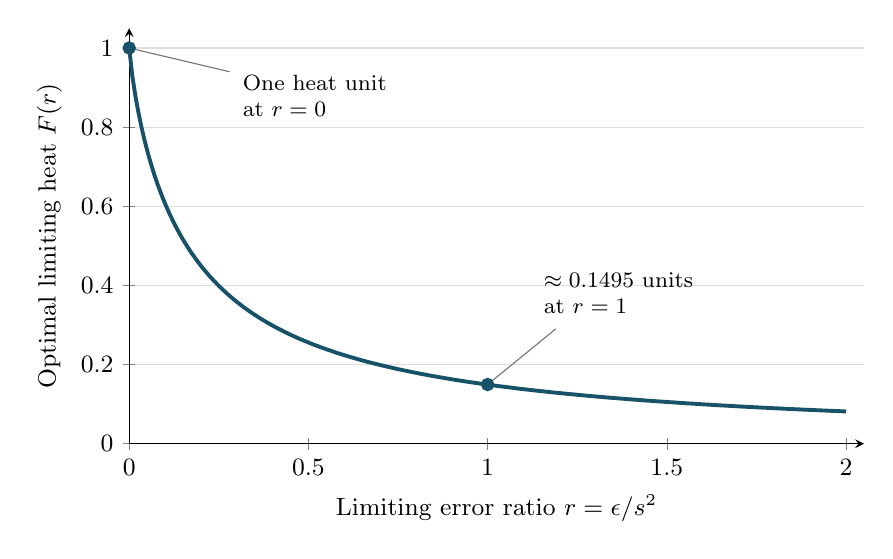
\begin{tikzpicture}
\begin{axis}[
 width=0.9\linewidth, height=2.7in,
 xmin=0,xmax=2.05, ymin=0,ymax=1.05,
 axis lines=left,
 xlabel={Limiting error ratio $r=\epsilon/s^2$},
 ylabel={Optimal limiting heat $F(r)$},
 xlabel style={font=\small},ylabel style={font=\small},
 tick label style={font=\small},
 xmajorgrids=false, ymajorgrids=true,
 grid style={black!13},
 xtick={0,0.5,1,1.5,2},ytick={0,0.2,0.4,0.6,0.8,1},
 every axis plot/.append style={line width=1.4pt},
 clip=false,
]
\addplot[teal,domain=0:2,samples=230] {1 + ((1+1/sqrt(1+4*x))/2)*ln((1+1/sqrt(1+4*x))/2)/ln(2) + (1-(1+1/sqrt(1+4*x))/2)*ln(max(0.000000001,1-(1+1/sqrt(1+4*x))/2))/ln(2)};
\addplot[only marks,mark=*,mark size=1.7pt,teal] coordinates {(0,1) (1,0.1495103748978384)};
\node[font=\footnotesize,anchor=west,align=left] at (axis cs:0.29,0.88) {One heat unit\\ at $r=0$};
\node[font=\footnotesize,anchor=west,align=left] at (axis cs:1.13,0.38) {$\approx 0.1495$ units\\ at $r=1$};
\draw[black!55,thin] (axis cs:0.28,0.94) -- (axis cs:0,1);
% Moderate-length leader stops below the label, clearing the r=1 equals sign.
\draw[black!55,thin] (axis cs:1.19,0.29) -- (axis cs:1,0.1495103748978384);
\end{axis}
\end{tikzpicture}
\end{center}

The optimal limiting heat decreases as the permitted error grows relative to squared overlap. Each point represents a joint positive-error limit, not an exact finite-device optimum. One heat unit is \(k_{\mathrm{B}}T\ln 2\).

The lower argument has no apparatus-dimension penalty, so it remains valid while the infimum ranges over larger and larger finite devices. For the upper argument, choose a finite recovery length separately at every stage. For example, at stage \(m\) choose \(M\) large enough that the recovery excess bound is below \(1/m\). Here \(m\) is a positive integer labelling the sequence. This produces finite devices whose excess heat tends to zero.

The theorem identifies a joint limiting law. It does not set \(q_{\min}(s,\epsilon) = F\left( \epsilon/s^{2} \right)\) at finite \(s\), and it does not determine a limit where \(s\) is held fixed.

\clearpage
\subsection{Why a full heat unit survives a vanishing average change}\label{subsec:surviving-heat}

\textbf{Preliminary.} Information can be held in correlations between two parts even if neither part's entropy tells the whole story. In a two-part entropy account, mutual information measures exactly the difference between the sum of the separate entropies and the joint entropy.

For the construction, the average output has Bloch vector \(( - s,0,0)\). Its eigenvalues are \((1 + s)/2\) and \((1 - s)/2\). The input average had entropy one bit. The system's entropy decrease is therefore \(J_{2}(s)\), which tends to zero as \(s \rightarrow 0\).

\Needspace{11\baselineskip}
After the bare collision the working bath qubit has entropy one, having started with entropy \(1 - J_{2}(b)\). Any fresh recovery qubits are still independent and unchanged, so their entropies cancel from the entropy-change calculation. Conservation of the total entropy shows that the final mutual information between system and complete bath is

\[I(S{:}B)' = J_{2}(b) - J_{2}(s).\]

The notation has the same meaning as \(I(A{:}B)'\) from Section~\ref{subsec:heat-bound}, with \(S\) replacing \(A\). The exact bath-only ledger can consequently be read as

\[q = J_{2}(s) + I(S{:}B)' + D_{2}\left( \rho\prime_{B}\|\gamma_{B} \right).\]

The three contributions are the system entropy decrease, final system--bath correlations, and bath departure from equilibrium. Recovery lowers the last toward zero while preserving the first two. The average-state entropy calculation sees only \(J_{2}(s)\). It misses the correlation contribution, which approaches \(F(r)\).

At \(r = 0\), the common limiting bias is one and

\[F(0) = 1 - h_{2}(1) = 1.\]

Thus the optimal mean heat approaches one full unit even though the system's average entropy decrease vanishes. In the full model with workspace, the necessary record concerns workspace and bath together; the bath-only correlation formula above describes the explicit construction.

Three different zeros must be kept separate:

\begin{center}
\begin{tabularx}{\linewidth}{@{}p{0.29\linewidth}X@{}}
\toprule
\textbf{Condition} & \textbf{Meaning}\\
\midrule
$s=0$ & The two targets are the original orthogonal inputs. The identity operation suffices.\\[3pt]
$\epsilon=0$ at fixed $0<s<1$ & Both nonorthogonal pure targets must be produced exactly. This is impossible in the finite returned-workspace model (Section~\ref{subsec:exact-output}).\\[3pt]
$r=0$ & Positive $s$ and positive $\epsilon$ approach zero with $\epsilon/s^2\to0$. Their heat infima approach one unit.\\
\bottomrule
\end{tabularx}
\end{center}

At every finite stage of the last case, the constructed bias remains below one. The Gibbs state stays full rank and the gap stays finite. Gaps and recovery lengths may nevertheless grow without a common bound along the sequence.

For larger finite \(r\), \(F(r)\) decreases because the allowed error is larger relative to the geometric scale. The curve itself tends to zero as \(r\) grows without bound. That property of the curve does not automatically prove a uniform theorem for every path with a divergent ratio \(\epsilon/s^{2}\).

\Needspace{16\baselineskip}
\section{Full-channel accuracy and exact-output limitations}\label{sec:consequences}

\Needspace{7\baselineskip}
\subsection{The same optimal heat under full-channel accuracy}\label{subsec:channel-accuracy}

\textbf{Preliminary.} A quantum channel describes an operation on every input state. Testing only \(\left| 0 \right\rangle\) and \(\left| 1 \right\rangle\) leaves its action on coherent combinations unspecified. A reference system is another quantum system that the device does not act on. It may be correlated or entangled with the input. Entanglement is a form of joint quantum correlation that cannot be expressed as a probabilistic mixture of separate product states.

Define the desired channel \(\mathcal{T}_{s}\) as follows: measure the input in the zero-or-one basis, then prepare \(\phi_{0}\) or \(\phi_{1}\) according to the answer. For an input matrix \(\rho\) with diagonal entries \(p_{0},p_{1}\), this means

\[\mathcal{T}_{s}(\rho) = p_{0}\phi_{0} + p_{1}\phi_{1}.\]

\Needspace{8\baselineskip}
Here \(p_{0},p_{1}\) refer to the input probabilities, not the earlier bath populations. The ideal channel discards the input off-diagonal entries. Let \(\mathcal{N}\) be the actual system channel. The stronger \textbf{half-diamond error} is written \(\tfrac{1}{2}\lVert\mathcal{N}-\mathcal{T}_{s}\rVert_{\diamond}\). It is the largest output trace distance over all input states, including inputs entangled with an untouched reference. The subscript diamond names this channel norm. The stronger task requires that error to be at most \(\epsilon\).

Any channel passing this stronger test passes the two branch tests. The reverse statement about an unmodified device need not hold. We instead construct a conversion.

Add a Gibbs qubit whose two energies are both zero. It is an equal mixture of its two basis states at the same temperature. Use it to apply either no phase change to the input or a sign change of the input's \(\left| 1 \right\rangle\) amplitude, each with equal probability. This is implemented coherently as one controlled unitary. Ignoring the extra qubit gives \textbf{dephasing}:

\[\mathcal{D}\left( \begin{pmatrix}
p & z \\
z^{*} & 1 - p
\end{pmatrix} \right) = \begin{pmatrix}
p & 0 \\
0 & 1 - p
\end{pmatrix}.\]

Dephasing removes the off-diagonal entry because the two possible phase operations give \(z\) and \(- z\), which cancel. Both original basis inputs are unchanged. Feed this dephased input to the original device. The converted channel is

\[\widetilde{\mathcal{N}}(\rho) = p_{0}\sigma_{0} + p_{1}\sigma_{1}.\]

The tilde identifies the converted channel. It has exactly the same two branch outputs, branch heat values, and average workspace return as the original device. The extra qubit has zero energy, so it adds zero charged heat. It remains a physical component and is included in the allowed finite Gibbs reservoir.

To check the stronger accuracy, let \(e_{x} = D\left( \sigma_{x},\phi_{x} \right)\). For an arbitrary input with a reference, let \(R_{x}\) be its unnormalized reference state associated with basis answer \(x\). Each \(R_{x}\) is positive and its trace is the corresponding probability; the two traces add to one. Dephasing removes the terms connecting the system's zero and one alternatives and leaves these two diagonal reference blocks. The ideal and converted channels attach their respective output states to the same blocks. Their output difference is therefore

\[\left( \sigma_{0} - \phi_{0} \right) \otimes R_{0} + \left( \sigma_{1} - \phi_{1} \right) \otimes R_{1}.\]

\Needspace{6\baselineskip}
The triangle inequality bounds its half trace norm by

\[e_{0}\operatorname{Tr} R_{0} + e_{1}\operatorname{Tr} R_{1} \leq \max\{ e_{0},e_{1}\}.\]

This uses the fact that multiplying a Hermitian difference by a positive reference state through a tensor product multiplies its trace norm by that state's trace. The eigenvalues of the tensor product are the pairwise products, which explains the rule. A basis input attaining the larger error gives the reverse bound. Thus

\[\frac{1}{2} \lVert \widetilde{\mathcal{N}} - \mathcal{T}_{s}\rVert_{\diamond} = \max\{ e_{0},e_{1}\}.\]

Let \(q_{\min}^{\diamond}(s,\epsilon)\) denote the heat infimum with this stronger accuracy condition. The two directions now give

\[q_{\min} \leq q_{\min}^{\diamond}\quad\text{and}\quad q_{\min}^{\diamond} \leq q_{\min},\]

so the two infima are exactly equal at every finite parameter pair in our stated domain. Their common value has the same limit \(F(r)\).

Heat and workspace return are still evaluated on the original equal-prior ensemble. The stronger accuracy test does not change the objective into worst-case heat over all inputs. A strict cap on reservoir size could forbid the additional qubit, in which case this conversion would no longer establish equality within that restricted class.

\Needspace{7\baselineskip}
\subsection{Why exactly pure targets are impossible in a finite device}\label{subsec:exact-output}

\textbf{Preliminary.} The support of a state is the space spanned by its directions with positive eigenvalues. Its rank is the number of those directions. Full rank means every direction is occupied. A unitary preserves rank and orthogonality of supports.

A pure marginal forces product form with the rest of the apparatus. To see why, choose the pure state as one basis direction. The joint state has zero probability in every orthogonal system direction. A valid density matrix must assign nonnegative probabilities to every measurement, including measurements of combinations of basis vectors. Consequently, the squared magnitude of an off-diagonal entry cannot exceed the product of its two diagonal probabilities. If either probability is zero, the connecting entry is zero too. Only the pure system direction remains, multiplied by some environment state. The environment itself need not be pure.

Suppose, for contradiction, that a finite allowed device produces both targets exactly for a fixed \(0 < s < 1\). Let the initial workspace rank be \(k\), and let the bath dimension be \(d_{B}\). Since the Gibbs bath has full rank, the initial environment rank is \(kd_{B}\).

Exact purity would force final branch states of the form

\[\rho\prime_{SAB,x} = \phi_{x} \otimes \omega_{x},\quad\quad \operatorname{rank}\omega_{x} = kd_{B}.\]

The notation \(\omega_{x}\) names the final environment state. Its rank follows because the complete unitary preserves the initial rank, and the pure system factor has rank one.

Now consider an initially empty workspace direction. Exact average return requires its final average probability to be zero. Both branch probabilities are nonnegative, so each must be zero. Positive probability in one branch cannot be canceled by a negative probability in the other. Thus neither environment branch can use any initially empty workspace direction.

Both \(\omega_{0}\) and \(\omega_{1}\) must therefore fit inside the same space: the \(k\) initially occupied workspace directions combined with all \(d_{B}\) bath directions. That space has dimension \(kd_{B}\). Each state also has rank \(kd_{B}\), so each fills the whole available space. Their supports cannot be orthogonal.

\Needspace{9\baselineskip}
But the complete input states were orthogonal because their system factors were \(\left| 0 \right\rangle\) and \(\left| 1 \right\rangle\). The same unitary must preserve that orthogonality. Since the final system factors have nonzero overlap \(s\), the final environment supports would have to be orthogonal. In formulas,

\[0 = \operatorname{Tr}\left( \rho\prime_{SAB,0}\rho\prime_{SAB,1} \right) = s^{2}\operatorname{Tr}\left( \omega_{0}\omega_{1} \right) > 0,\]

which is impossible. The strict positivity follows because both environment states are positive on the same full support. They need not be identical to have a positive overlap.

This proof permits a rank-deficient nonthermal workspace, different branch workspace marginals, and correlations within workspace and bath. Enlarging either finite system does not remove the contradiction: each environment branch still fills the entire available supported space.

The exactly zero-error task is therefore infeasible. This is not a statement that a device releases infinite heat. It says that no such finite device exists. Positive errors can nevertheless approach zero along a sequence, allowing the optimal limiting heat from Section~\ref{subsec:optimal-crossover} to be approached. For example, \(s_{m} = 1/m\) and \(\epsilon_{m} = 1/m^{3}\) have positive errors and ratio \(1/m \rightarrow 0\) for integers \(m \geq 2\).

\Needspace{10\baselineskip}
\section{Finite evidence and the complete result}\label{sec:evidence}

\Needspace{7\baselineskip}
\subsection{A finite comparison of strict and relaxed precision}\label{subsec:finite-comparison}

\textbf{Preliminary.} A lower bound describes every compliant device. An upper bound can come from one working device. If the lower bound for one task exceeds the cost of a construction for another, their optimal costs are separated even if neither optimum is known exactly.

Fix the target overlap at \(s = 0.05\) and compare two permitted errors. All values below are theoretical calculations in the same heat units.

\begin{center}
\begin{tabularx}{\linewidth}{@{}p{0.35\linewidth}X@{}}
\toprule
\textbf{Accuracy requirement} & \textbf{Established heat statement}\\
\midrule
Strict error $\epsilon=0.0001$ & Every allowed device with exact average workspace return has heat at least about $0.498044$.\\[3pt]
Relaxed error $\epsilon=0.0025$ & The bare two-qubit construction has heat about $0.311485$.\\
\bottomrule
\end{tabularx}
\end{center}

The relaxed device starts with bath probabilities approximately \(0.723943\) and \(0.276057\). Its energy gap is
\[\frac{\Delta}{k_{\mathrm{B}}T}\approx 0.964105468.\]
The final average upper-level probability is one half. Multiply its increase by the gap, then convert to our heat units:

\[q = \frac{(0.5 - 0.276057) \times 0.964105468}{\ln 2} \approx 0.311485.\]

The division by \(\ln 2\) is needed because the quoted gap was in units of \(k_{\mathrm{B}}T\). The common sideways component of both system outputs remains exactly correct. This comparison uses no recovery sequence.

\Needspace{9\baselineskip}
Let \(q_{\mathrm{strict}}\) and \(q_{\mathrm{relaxed}}\) be the two optimal heat infima. Let \(L_{\mathrm{strict}}\) denote the strict finite lower bound, and let \(q_{\mathrm{device}}\) be the relaxed construction's heat. The logical statement is

\[q_{\mathrm{strict}} \geq L_{\mathrm{strict}} > q_{\mathrm{device}} \geq q_{\mathrm{relaxed}}.\]

Thus relaxing the specified error really permits a strictly lower optimal heat cost. Neither displayed number is asserted to equal a finite optimum.

The separation survives a modest workspace allowance. For a strict device with a 16-level workspace whose average marginal returns within trace distance \(0.0001\), the entropy allowance derived in Section~\ref{subsec:heat-bound} is about \(0.001864\) bits. Its lower heat bound is still about \(0.496180\), above the relaxed construction's cost. The allowance applies to the whole workspace state.

\Needspace{7\baselineskip}
\subsection{What the result adds and which cost it determines}\label{subsec:contribution}

\textbf{Preliminary.} Two thermodynamic claims can use different tasks, accuracy measures, or resource accounts. A work cost assigned to a battery, or a work rate obtained by collectively processing many inputs, is not automatically the heat cost for one input in this apparatus model.

The familiar ingredients used here include unitary information preservation, entropy inequalities, the Gibbs heat identity, and recovery through thermal interactions. The contribution is their combination for this specific conditional task: individual output accuracy forces an environmental record; the record gives a bound uniform in apparatus size; a fully counted construction reaches the same limiting curve.

Each piece is necessary. An average-state entropy calculation misses the two individual requirements. A working device alone supplies no universal lower bound. A lower bound alone does not establish an optimum. The matching curve follows because both directions have been proved for the same task and the same resource model.

The cost determined here is mean reservoir heat for one processed input. Under the specified boundary conditions, it also equals mean supplied work. Those conditions set the system's energy to zero at the start and end, switch interactions off at those boundaries, and keep the bath and workspace energy assignments unchanged. The energy balance is

\[W = Q + \Delta E_{A}.\]

Here \(W\) is net mean work supplied by the drive and \(\Delta E_{A}\) is the workspace's final-minus-initial mean energy. Exact average workspace return gives \(\Delta E_{A} = 0\), so \(W = Q\). If the workspace energy changes, that change must be included before translating a heat bound into a work bound.

The result identifies precision as a physical cost parameter that can remain important when average entropy loss is small. It gives an exact limiting optimum and a finite theoretical separation. A hardware performance estimate would additionally need the costs of source preparation, controller construction, duration, and control accuracy. The optimization permits finite devices whose sizes and gaps grow along the sequence; it supplies no uniform cap on those resources.

\clearpage
\subsection{The complete result as one argument}\label{subsec:summary}

\textbf{Preliminary.} The conclusion has two logically different parts: what no compliant device can beat, and what a sequence of compliant finite devices can approach. An equality of their limits follows only because the lower bound and the construction use the same assumptions.

\Needspace{11\baselineskip}
The physical question is simple to state. A device receives one of two perfectly distinguishable inputs without being told which. It must return the corresponding nearly orthogonal pure target within a specified error. The same fixed reversible operation acts on the input, an initially independent workspace, and an initially thermal reservoir. Every thermal component is counted. The workspace must return exactly on its average marginal for the equally likely inputs.

Target coherence is of size \(s\), while the associated probability change is of size \(s^{2}\). These two accuracy requirements force the comparison environment states to differ. The information inequality and disturbance estimate turn that difference into a necessary record in the actual environment, with a bound independent of apparatus size.

Nearly pure system outputs retain little entropy within either branch. The environment must therefore acquire entropy. The Gibbs identity converts that increase into heat, while explicitly charging any workspace entropy consumed. This proves a finite lower bound for every allowed device.

A thermal qubit supplies matching outputs. Recovery through a finite sequence of additional Gibbs qubits removes avoidable excess cost, while every spent component and every correlation stays inside the account. The recovered construction and the universal lower bound approach the same value.

\Needspace{10\baselineskip}
\subsubsection{The result in one formula}\label{the-result-in-one-formula}

Let \(s\) be the overlap magnitude of the two pure targets, \(\epsilon\) the maximum permitted trace-distance error on either output, and \(q_{\min}\) the optimal mean heat infimum in units of \(k_{\mathrm{B}}T\ln 2\). If \(s \rightarrow 0\), every finite-stage error is positive, and \(\epsilon/s^{2} \rightarrow r\) for a finite \(r \geq 0\), then

\[q_{\min}(s,\epsilon) \rightarrow 1 - h_{2}\left( \frac{1 + (1 + 4r)^{- 1/2}}{2} \right),\]

where \(h_{2}(p) = - p\log_{2}p - (1 - p)\log_{2}(1 - p)\) is binary entropy and zero-probability terms are zero. Requiring an error much smaller than \(s^{2}\) gives \(r = 0\) and a limiting cost of one heat unit. At \(r = 1\), the limiting cost is approximately \(0.149510\) units.

\Needspace{5\baselineskip}
\subsubsection{The consequences that belong with the formula}\label{the-consequences-that-belong-with-the-formula}

The finite lower bound applies before taking a limit and charges consumed workspace entropy. The stronger channel test, including reference-entangled inputs, has the same heat infimum: physical dephasing converts each branch-feasible device without changing its equal-prior heat. Producing both nonorthogonal pure targets exactly is impossible for a finite apparatus with a full-rank Gibbs bath and exact average workspace return.

At the same overlap, the finite benchmark also proves that a relaxed construction costs less than every device satisfying the stricter tolerance.

The assumptions matter. Always preparing the average target gives either branch error \(\sqrt{1 - s^{2}}/2\), approaching one half. Leaving the label in fresh pure workspace consumes a resource. Fixed hardware caps may exclude the construction or the channel conversion. Such tasks require their own resource account.

Individually precise outputs can therefore impose a finite heat cost while their average change vanishes. Under the stated model, the exact limiting cost is set by error divided by squared target overlap.


\end{document}
